\label{chap:modeling}

\section{Modeling technique}
The purpose of this assignment is to perform a market basket analysis using the technique
association rule mining. This technique discovers frequent patterns, which form relations
between items in the dataset, and are then expressed as association rules. The rules will
be of the form: If customer buys product A, the customer is likely to also buy product B.
The rule comes with a certain support (frequence of an item or itemset in the entire dataset)
and confidence (the probability to find product B in a basket already containing product A), which 
quantifies its strength ~\cite[Ch.~5, Sec.~5.2]{courseLitt}.

The structured dataset consists of 94 unique items and over 20,000 entries in about 9,000 transactions.
This technique is suitable for this task since the dataset consists of transactional data with
multiple items per basket and we will be able to analyse any existing relations between
transactions (baskets) and items. 

The technique of association rule mining was implemented in Altair RapidMiner ~\cite{RapidMiner} using a combination
of operators FP-Growth and Create Association Rules and in Knime ~\cite{Knime} using node Association Rule Learner.
Identical input and configuration of support-, and confidence level was used in both tools to be
able to analyse the outcome and find similarity and differences between the two.

\section{Modeling process}
The Bakery Transaction dataset csv-file was imported into RapidMiner with the operator Retrieve
followed by Select Attributes. The operator Aggregate transforms the entries for every item into
a baskets with a collection of items with the same transaction number. When the baskets are formed
the attribute TransactionNo is no longer useful and therefore excluded in a second Select Attributes
to complete the preprocessing, keeping only the aggregated baskets for analyse. This step prepared 
the data for association rule mining in line with preprocessing requirements discussed in 
~\cite[Ch.~3, Sec.~3.3]{courseLitt}. The operator FP-Growth identifies frequent patterns among the basket content, 
depending on the configurated support and finally the operator Create Association Rules, forms rules for 
the relation between items, depending on the configured confidence ~\cite[Ch.~5, Sec.~5.2]{courseLitt}.

\begin{figure}[H]
\centering
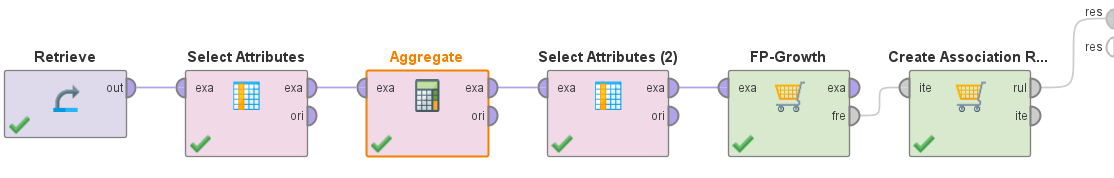
\includegraphics[width=0.8\textwidth]{figures/AssociationRulesRapidMinerProcess.png}
\caption{RapidMiner process for association rule mining.}
\label{fig:AssociationRulesRapidMinerProcess}
\end{figure}

The Knime process is very similar and starts with the node CSV-Reader followed by Column filter,
selecting TransactionNo and Items. The node GroupBy transforms the entries into baskets and last
the node Association Rule Learner forms the rules. Support and confidence are configurated in the
last node.

\begin{figure}[H]
\centering
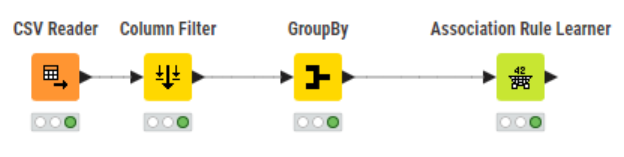
\includegraphics[width=0.8\textwidth]{figures/AssociationRulesKnimeProcess.png}
\caption{Knime process for association rule mining.}
\label{fig:KnimeProcess}
\end{figure}

\section{Modeling results}
We tested three different support values combined with a fixed confidence value to determine which
one was most appropriate to use, giving a reasonable number of association rules. As Tan et 
al. ~\cite[Ch.~5, Sec.~5.3]{courseLitt} emphasize, selecting appropriate thresholds for support and confidence 
is a critical part of association rule mining

Confidence (fixed): 0,5
Support:
0,1 --\textgreater 8 rules (too few, all relations expected)
0,01 --\textgreater 17 rules (most reasonable in this case)
0,001 --\textgreater 72 rules (too many, any relation considered a rule)

Keeping the support value fixed at 0,01 and varying the confidence within the range 0,5 - 0,7.
With values higher than 0,7 there were very few rules left, especially for Knime which seems to
find fewer association rules compared to RapidMiner when increasing the confidence value.

The rules in table \ref{tab:rapidminer_rules} show the output from RapidMiner with
support 0,01 and confidence 0,6. And table \ref{tab:knime_rule} shows the output from Knime with
the same support and confidence values. The rule found in both tools is that if a customer buys
Toast, the customer is likely to also buy Coffee. The support value of 0,024 means that 2,4\%
of all transactions contain both items and the confidence value of 0,704 means that in 70,4\%
of the transactions containing Toast, Coffee is also present.

\begin{table}[H]
\centering
\caption{Association rules with support and confidence values}
\begin{tabular}{l l r r}
\hline
\textbf{Conditions} & \textbf{Consequent} & \textbf{Support} & \textbf{Confidence} \\
\hline
Cake, Hot chocolate & Coffee & 0.007 & 0.602 \\
Salad               & Coffee & 0.007 & 0.626 \\
Toast               & Coffee & 0.024 & 0.704 \\
Keeping It Local    & Coffee & 0.005 & 0.810 \\
\hline
\end{tabular}
\label{tab:rapidminer_rules}
\end{table}

\begin{table}[H]
\centering
\caption{Association rule generated in KNIME}
\begin{tabular}{l l r r r}
\hline
\textbf{Conditions} & \textbf{Consequent} & \textbf{Support} & \textbf{Confidence} \\
\hline
Toast & Coffee & 0.024 & 0.704 \\
\hline
\end{tabular}
\label{tab:knime_rule}
\end{table}

\section{Challenge and limitation}

\begin{itemize}
    \item Finding the right balance between support and confidence to get a reasonable number of rules
    to analyse can be challenging. Too few rules and we might miss important relations, too many rules
    and we might end up with relations that are not relevant.
    
    \item Items appearing in many transactions will form many rules with other items, but the relation
    might not be that interesting.
    
    \item There are more than one way to build the process in both RapidMiner and Knime, and
    different ways might lead to different results.

    \item Association rule mining identifies relations between items, but does not necessarily prove causation
    or explain why the relation exists.
\end{itemize}
